\chapter{Ход работы}

\textbf{Цель работы}: провести модельное исследование однополупериодного выпрямителя с фильтром при использовании диода \textbf{S2GА}.

Исходные данные: условия (дано) из домашнего задания и результаты расчетов.

\begin{figure}[h!]
	\centering
	\caption{Схема однополупериодного выпрямителя}
	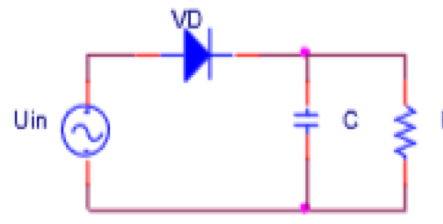
\includegraphics{images/scheme1.png}
\end{figure}

\begin{figure}[h!]
	\centering
	\caption{Модель в OrCAD}
	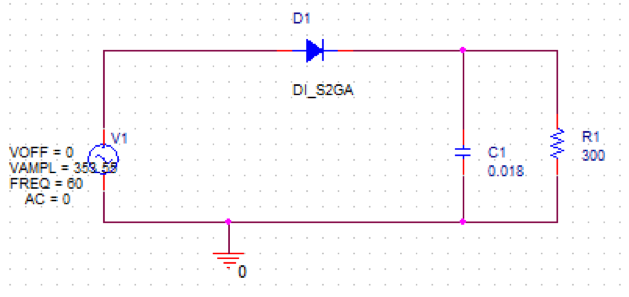
\includegraphics{images/scheme2.png}
\end{figure}

\newpage
\section{Результаты моделирования}

\begin{figure}[h!]
	\centering
	\caption{Входное напряжение (зеленый, В), выходное напряжение (красный, В)}
	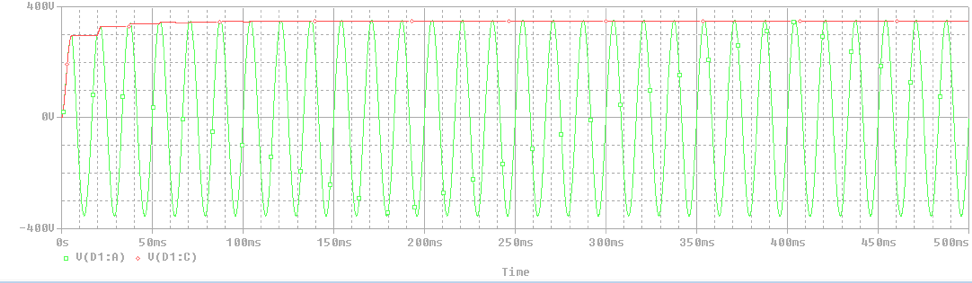
\includegraphics{images/model1.png}
\end{figure}


\begin{figure}[h!]
	\centering
	\caption{Ток на нагрузке (синий, А), средний ток на нагрузке (красный, А)}
	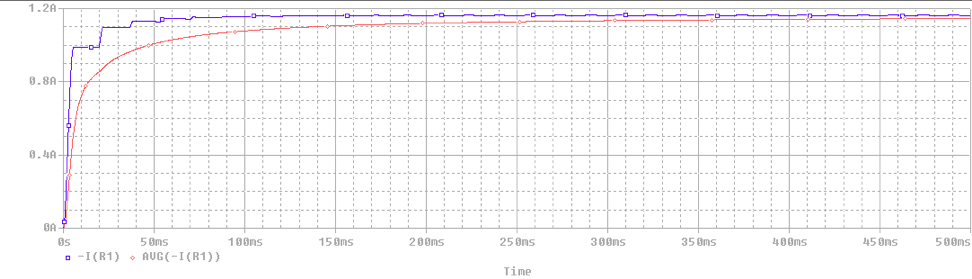
\includegraphics{images/model2.png}
\end{figure}

\begin{figure}[h!]
	\centering
	\caption{Ток через диод (синий, А), максимальное значение тока через диод (красный, А)}
	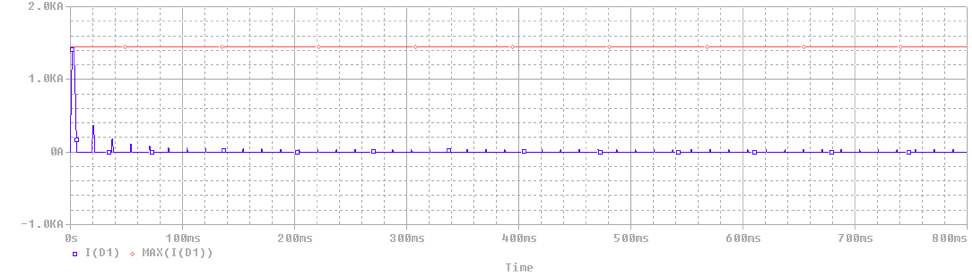
\includegraphics{images/model3.png}
\end{figure}

\section{Измерения в OrCAD}

Среднее напряжение на нагрузке, В:
\[
U_{L\_AVG\_EXP} = 348.8095 
\]

Cредний ток на нагрузке, А:

\[
I_{L\_AVG\_EXP}= 1.1454
\]

Амплитуда пульсаций, В:   

\[
\Delta U_{B\_EXP}=1.025
\]

Коэффициент пульсаций:
\[
K_{p\_EXP}=0.001039
\]

Бросок зарядного тока диода, А: 
\[
I_{VD\_ON\_EXP}= 1443.3
\]

Максимальный ток диода, А: 
\[
I_{VD\_MAX\_EXP} = 26,803 
\] 

\section{Расчёт погрешностей}

Погрешность $U_{L\_AVG}$:

\[
U_{L\_AVG}=\left | \frac{U_{L\_AVG\_EXP}-U_{L\_AVG}}{U_{L\_AVG}} \right | = 7.1 \%
\]


Погрешность $I_{L\_AVG}$:

\[
I_{L\_AVG}=\left | \frac{I_{L\_AVG\_EXP}-I_{L\_AVG}}{I_{L\_AVG}} \right |= 7.9 \%
\]

Погрешность $\Delta U_B$: 

\[
\Delta U_B=\left | \frac{\Delta U_{B\_EXP}-\Delta U_B}{\Delta U_B} \right |= 2.5 \%
\]

Погрешность $K_p$:

\[
K_p=\left | \frac{K_{p\_EXP}-K_p}{K_p} \right |= 1.7 \%
\]


Погрешность $I_{VD\_ON}$:
\[
I_{VD\_ON} =\left |  \frac{I_{VD\_ON\_EXP}-I_{VD\_ON}}{I_{VD\_ON}}\right |=7.3 \%
\]

Погрешность $I_{VD\_MAX}$:
\[
I_{VD\_MAX}=\left |  \frac{I_{VD\_MAX\_EXP}-I_{VD\_MAX}}{I_{VD\_MAX}} \right |=2.1 \%
\]

\chapter{Вывод}

В ходе выполнения лабораторной работы был спроектирован и промоделирован однополупериодный выпрямитель с фильтром, построены графики изменения величин в OrCAD PSpice, измерены необходимые величины по этим графикам и рассчитаны погрешности.

Ни одна из вычисленных погрешностей не превышает 10\%, что свидетельствует о корректности выполнения работы и соответствии модели расчетным значениям.